\documentclass[dvipsnames]{beamer}

\usetheme{Dresden}
\usecolortheme{dove}
\setbeamertemplate{navigation symbols}{}
\usefonttheme{professionalfonts}

\usepackage[utf8]{inputenc}
\usepackage[T1]{fontenc}
\usepackage{lmodern}

\usepackage{amsmath}
\usepackage{amssymb}
\usepackage{amsfonts}
\usepackage{bm}
\usepackage{float}
\usepackage{graphicx}
\usepackage{tabulary}
\usepackage{longtable}

% \usepackage[]{xcolor}
\usepackage{tikz}
\usetikzlibrary{arrows,decorations.pathmorphing,backgrounds,positioning,fit,petri,decorations.pathreplacing}
\tikzset{circly/.style={draw,circle,minimum size=1cm},
    arraycell/.style={draw,rectangle,minimum size=1cm,node distance=0},
    accolade/.style={decorate,decoration={brace,amplitude=10pt}},
    enoughdamnvspace/.style={font=\vphantom{$ f $}},
    smallnode/.style={circle,fill,inner sep=0,minimum size=5pt}
}
\usepackage{pgfplots, pgfplotstable}
\pgfplotsset{compat=1.16}
\pgfplotsset{legend style={fill opacity=0.7,text opacity=1}}
\pgfplotsset{cycle list={
    {thick,MidnightBlue,mark=*},
    {mark options=solid,dashed,thick,OrangeRed,mark=square*},
    {thick,YellowOrange,mark=diamond*},
    {thick,Fuchsia,mark=asterisk},
    {mark options=solid,dashed,thick,ForestGreen,mark=x},
    {thick,Turquoise,mark=square*},
    {Black,mark=triangle*},
    {mark options=solid,dashed,thick,RedViolet,mark=diamond*},
    {LimeGreen,mark=square*}
}}
\pgfplotsset{axis lines=left}

\usepackage{algorithm}
\usepackage{algorithmicx}
\usepackage[noend]{algpseudocode}

\renewcommand{\sfdefault}{phv}
\renewcommand{\rmdefault}{bch}
\def\mytablesize{\small}

\frenchspacing


\newcommand{\sequencetickmarks}[3]
{
% args: (number of tick marks, x of first tick mark, y of first tick mark)
    \pgfmathsetmacro\secondtickmark{#2+0.5}
    \pgfmathsetmacro\lasttickmark{#2+0.5*#1}

    \draw (#2,#3) -- (\lasttickmark,#3);

    \foreach \x in {#2,\secondtickmark,...,\lasttickmark}
        \draw (\x,#3) -- +(0,3pt);
}

\newcommand{\sequenceeventtypes}[4]
{
% args: (x of first event, y, t of first event, list of t/A pairs)
    \pgfmathsetlengthmacro\nodeheight{(#2)+(.8em)}

    \foreach \t/\eventtype [evaluate=\t as \x using (\t-#3)*0.5+(#1)] in {#4}
    {
        \node [font=\vphantom{$ fbd $}] at (\x,#2) {$ \eventtype $};
        \node (t\t) [inner sep=0] at (\x,\nodeheight) {};
    }
}

\newcommand{\windowthingy}[2]
{
% args: starting position (leftmost point of horizontal line), number of timestamps
    \pgfmathsetmacro\windowthingylength{#2*0.5-0.1}
    \draw [thick] #1 ++(0,3pt) -- ++(0,-3pt) -- ++(\windowthingylength,0) -- ++(0,3pt);
}

\newcommand{\examplesequence}
{
    \sequencetickmarks{23}{-5.5}{0}

    \sequenceeventtypes{-5.5}{1em}{30}{32/c,33/f,34/b,35/b,38/c,40/d,41/a,44/b,46/e,47/a,48/e,49/c};
}

\newcommand{\examplesequencetimestamps}
{
    \foreach \x [evaluate=\x as \timestamp using int((\x*2)+41)] in {-5.5,-3,...,5.5}
    \node at (\x,-1em) {$ \timestamp $};
}

\begin{document}

\title{Evaluation of Algorithms for Sequential Pattern Mining in Long Event Sequences}
\author{Josse Coen}
\date{6 September 2018}

\frame{\titlepage}

\begin{frame}
\frametitle{Event sequences}

\begin{align*}
\Sigma = \{ a, b, c, d, e, f \}
\end{align*}

\begin{center}
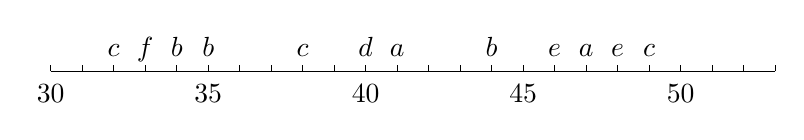
\begin{tikzpicture}[scale=0.8]

\examplesequence
\examplesequencetimestamps

\end{tikzpicture}
\end{center}

\end{frame}
\begin{frame}
\frametitle{Window on a sequence}

\begin{center}
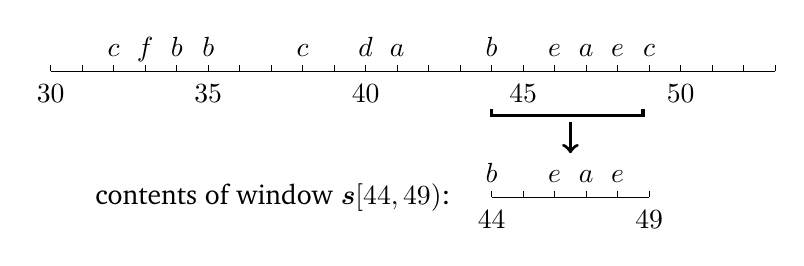
\begin{tikzpicture}[scale=0.8]

\examplesequence
\examplesequencetimestamps

\draw [very thick] (1.5,-0.6) -- ++(0,-3pt) -- ++(2.4,0) -- ++(0,3pt);

\draw [->,very thick] (2.75,-0.8) -- ++(0,-0.5);

\draw (1.5,-2) -- ++(2.5,0);

\foreach \x in {1.5,2,...,4}
    \draw (\x,-2) -- ++(0,3pt);

\foreach \x/\label in {
    1.5/b,
    2.5/e,
    3/a,
    3.5/e}
    \path (\x,-2) ++(0,1em) node [enoughdamnvspace] {$ \label $};

\path (1.5,-2) ++(0,-1em) node {$ 44 $};
\path (4,-2) ++(0,-1em) node {$ 49 $};

\node [anchor=east] at (1,-2) {contents of window $ \boldsymbol{s}[44,49) $:};

\end{tikzpicture}
\end{center}

\end{frame}
\begin{frame}
\frametitle{Episodes}

labelled directed acyclic graph

\begin{align*}\alpha=(V, E, lab)\end{align*}

\begin{itemize}
\item $ (V, E) $ directed acyclic graph
\item $ lab : V \to \Sigma $ mapping of nodes to event types
\end{itemize}

\end{frame}
\begin{frame}
\frametitle{Parallel episodes}

\begin{itemize}
\item all episodes $ (V, E, lab) $ for which $ E = \emptyset $
\item notation: \begin{align*} \{ A_1, A_2, \ldots, A_n \} \end{align*} with $ A_i $ event types
\end{itemize}

\end{frame}
\begin{frame}

\begin{center}
\begin{tikzpicture}[scale=1.5]
\node (parB) at (3,2.6) [smallnode,label={$ b $}] {};
\node (parE1) at (2,1.8) [smallnode,label={$ e $}] {};
\node (parE2) at (4.5,2.4) [smallnode,label={$ e $}] {};
\node (parC) at (3.5,2) [smallnode,label={$ c $}] {};
\end{tikzpicture}
\end{center}

\end{frame}
\begin{frame}
\frametitle{Serial episodes}

\begin{itemize}
\item all episodes $ (V, E, lab) $ for which $ E $ defines total order on $ V $
\item notation: \begin{align*} A_1 \to A_2 \to \cdots \to A_n \end{align*} with $ A_i $ event type corresponding to $ i $-th node
\end{itemize}

\end{frame}
\begin{frame}

\begin{center}
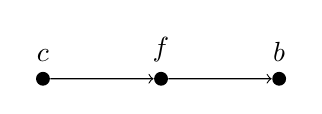
\begin{tikzpicture}[scale=1.5]
\node (serC) at (-5,2.5) [smallnode,label={$ c $}] {};
\node (serF) at (-4,2.5) [smallnode,label={$ f $}] {};
\node (serB) at (-3,2.5) [smallnode,label={$ b $}] {};

\draw [->] (serC) -- (serF);
\draw [->] (serF) -- (serB);
\end{tikzpicture}
\end{center}

\end{frame}
\begin{frame}
\frametitle{Occurrences}

\begin{center}
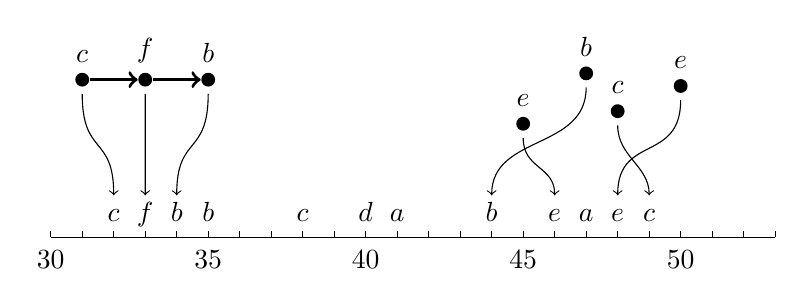
\begin{tikzpicture}[scale=0.8]

\examplesequence
\examplesequencetimestamps

% serial episode

\node (serC) at (-5,2.5) [smallnode,label={$ c $}] {};
\node (serF) at (-4,2.5) [smallnode,label={$ f $}] {};
\node (serB) at (-3,2.5) [smallnode,label={$ b $}] {};

\draw [->,very thick] (serC) -- (serF);
\draw [->,very thick] (serF) -- (serB);

\draw [->] ([yshift=-3pt]serC.south) .. controls +(0,-1) and +(0,1) .. (t32);
\draw [->] ([yshift=-3pt]serF.south) .. controls +(0,-1) and +(0,1) .. (t33);
\draw [->] ([yshift=-3pt]serB.south) .. controls +(0,-1) and +(0,1) .. (t34);

% parallel episode

\node (parB) at (3,2.6) [smallnode,label={$ b $}] {};
\node (parE1) at (2,1.8) [smallnode,label={$ e $}] {};
\node (parE2) at (4.5,2.4) [smallnode,label={$ e $}] {};
\node (parC) at (3.5,2) [smallnode,label={$ c $}] {};

\draw [->] ([yshift=-3pt]parB.south) .. controls +(0,-1) and +(0,1) .. (t44);
\draw [->] ([yshift=-3pt]parE1.south) .. controls +(0,-0.5) and +(0,0.5) .. (t46);
\draw [->] ([yshift=-3pt]parE2.south) .. controls +(0,-1) and +(0,1) .. (t48);
\draw [->] ([yshift=-3pt]parC.south) .. controls +(0,-0.5) and +(0,0.5) .. (t49);

\end{tikzpicture}
\end{center}

\end{frame}
\begin{frame}
\frametitle{Parallel episodes: array representation}

\begin{center}
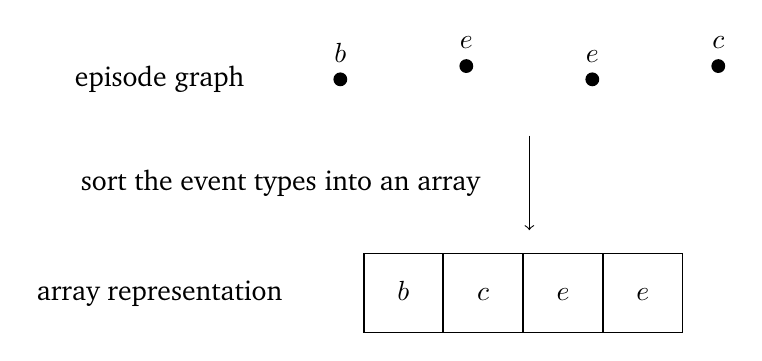
\begin{tikzpicture}[scale=0.8]

\node (n 1) [smallnode,label=above:$ b $] at (-3,-3pt) {};
\node (n 2) [smallnode,label=above:$ e $] at (-1, 3pt) {};
\node (n 3) [smallnode,label=above:$ e $] at ( 1,-3pt) {};
\node (n 4) [smallnode,label=above:$ c $] at ( 3, 3pt) {};

\node (episodegraphtext) [left=of n 1] {episode graph};

\draw [->] (0,-1) -- node [left=0.5cm] {sort the event types into an array} +(0,-1.5);

\node (a 1) [arraycell,enoughdamnvspace] at (-2,-3.5) {$ b $};
\node (a 2) [arraycell,right=of a 1,enoughdamnvspace] {$ c $};
\node (a 3) [arraycell,right=of a 2,enoughdamnvspace] {$ e $};
\node (a 4) [arraycell,right=of a 3,enoughdamnvspace] {$ e $};

\node at (episodegraphtext |- a 1) {array representation};

\end{tikzpicture}
\end{center}

\end{frame}
\begin{frame}

\begin{center}
\begin{tikzpicture}[scale=0.8]

\node (n 1) [smallnode,label=above:$ c $] at (-3,0) {};
\node (n 2) [smallnode,label=above:$ f $] at (-1,0) {}
    edge [pre] (n 1);
\node (n 3) [smallnode,label=above:$ b $] at (1, 0) {}
    edge [pre] (n 2);
\node (n 4) [smallnode,label=above:$ b $] at (3, 0) {}
    edge [pre] (n 3);

\node [left=of n 1] {episode graph};

\draw [->] (0,-1) -- node [left=0.5cm,align=right] {store event types into array,\\preserving topological ordering} +(0,-1.5);

\node (a 1) [arraycell,enoughdamnvspace] at (-2, -3.5) {$ c $};
\node (a 2) [arraycell,right=of a 1,enoughdamnvspace] {$ f $};
\node (a 3) [arraycell,right=of a 2,enoughdamnvspace] {$ b $};
\node (a 4) [arraycell,right=of a 3,enoughdamnvspace] {$ b $};

\node at (episodegraphtext |- a 1) {array representation};

\end{tikzpicture}
\end{center}

\end{frame}
\begin{frame}
\frametitle{Subepisode relationship}

\begin{align*}
\alpha \subseteq \beta \iff \text{ all sequences that cover } \beta \text{ also cover } \alpha
\end{align*}

\end{frame}
\begin{frame}
\frametitle{Fixed-window frequency}

Given window width $ \rho $, sequence $ \boldsymbol{s} $:
\begin{align*}
fr_f(\alpha, \boldsymbol{s}) = | \{ \boldsymbol{s}[t, t + \rho) \mid \boldsymbol{s}[t, t + \rho) \text{ covers } \alpha \} |
\end{align*}

\end{frame}
\begin{frame}
\frametitle{Minimal windows}

$ [a, b) $ minnimal window of $ \alpha $ if
\begin{itemize}
\item $ b - a \leq \rho $ for some $ \rho $
\item $ \nexists [c, d) \subset [a, b) : \boldsymbol{s} \text{ covers } \alpha $
\end{itemize}

\end{frame}
\begin{frame}

\begin{center}
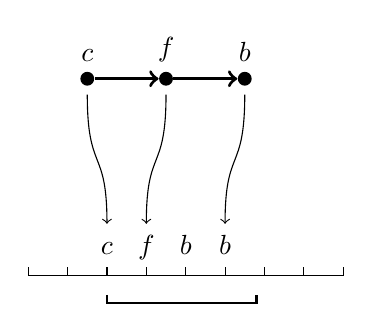
\begin{tikzpicture}

\sequencetickmarks{8}{-5.5}{0}
\sequenceeventtypes{-5.5}{1em}{30}{32/c,33/f,34/b,35/b}

% \foreach \x [evaluate=\x as \timestamp using int((\x*2)+41)] in {-5.5,-5,...,-1.5}
%     \node (t\timestamp) [inner sep=0] at (\x,1.8em) {};

%% draw occurrence proofs again
% serial episode

\node (serC) at (-4.75,2.5) [smallnode,label={$ c $}] {};
\node (serF) at (-3.75,2.5) [smallnode,label={$ f $}] {};
\node (serB) at (-2.75,2.5) [smallnode,label={$ b $}] {};

\draw [->,very thick] (serC) -- (serF);
\draw [->,very thick] (serF) -- (serB);

\draw [->] ([yshift=-3pt]serC.south) .. controls +(0,-1) and +(0,1) .. (t32);
\draw [->] ([yshift=-3pt]serF.south) .. controls +(0,-1) and +(0,1) .. (t33);
\draw [->] ([yshift=-3pt]serB.south) .. controls +(0,-1) and +(0,1) .. (t35);

% windows

\windowthingy{(-4.5,-10pt)}{4}

\end{tikzpicture}
\end{center}

\end{frame}
\begin{frame}

\begin{center}
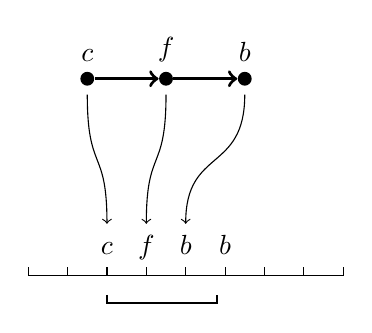
\begin{tikzpicture}

\sequencetickmarks{8}{-5.5}{0}
\sequenceeventtypes{-5.5}{1em}{30}{32/c,33/f,34/b,35/b}

\node (serC) at (-4.75,2.5) [smallnode,label={$ c $}] {};
\node (serF) at (-3.75,2.5) [smallnode,label={$ f $}] {};
\node (serB) at (-2.75,2.5) [smallnode,label={$ b $}] {};

\draw [->,very thick] (serC) -- (serF);
\draw [->,very thick] (serF) -- (serB);

\draw [->] ([yshift=-3pt]serC.south) .. controls +(0,-1) and +(0,1) .. (t32);
\draw [->] ([yshift=-3pt]serF.south) .. controls +(0,-1) and +(0,1) .. (t33);
\draw [->] ([yshift=-3pt]serB.south) .. controls +(0,-1) and +(0,1) .. (t34);

\windowthingy{(-4.5,-10pt)}{3}

\end{tikzpicture}
\end{center}

\end{frame}

\end{document}
